% =============================================================================
%  main_paper.tex
%  Journal Paper — IEEE Transactions on Power Delivery style
%
%  Title: Real-Time Inverse Parameter Estimation for Adaptive Overcurrent
%         Protection of Synchronous Generators
%
%  Target: IEEE Transactions on Power Delivery / IET Generation, Transmission
%          & Distribution
%
%  Compile:
%    pdflatex main_paper && bibtex main_paper &&
%    pdflatex main_paper && pdflatex main_paper
% =============================================================================

\documentclass[journal, twoside, 10pt]{IEEEtran}

% ---- Essential packages -----------------------------------------------------
\usepackage[T1]{fontenc}
\usepackage[utf8]{inputenc}
\usepackage{mathptmx}
\usepackage{microtype}

% ---- Mathematics ------------------------------------------------------------
\usepackage{amsmath, amssymb, mathtools}
\usepackage{bm}
\usepackage{siunitx}
\sisetup{detect-all, per-mode=symbol, range-phrase=\,--\,}

% ---- Figures and tables -----------------------------------------------------
\usepackage{graphicx}
\usepackage{subcaption}
\usepackage{booktabs}
\usepackage{array}
\usepackage{multirow}
\usepackage{float}

% ---- References and links ---------------------------------------------------
\usepackage[colorlinks=false]{hyperref}
\usepackage{xcolor}
\bibliographystyle{IEEEtran}

% ---- Algorithm --------------------------------------------------------------
\usepackage{algorithm}
\usepackage{algpseudocode}
\renewcommand{\algorithmicrequire}{\textbf{Input:}}
\renewcommand{\algorithmicensure}{\textbf{Output:}}

% ---- Theorem environments ---------------------------------------------------
\usepackage{amsthm}
\newtheorem{proposition}{Proposition}
\newtheorem{remark}{Remark}

% ---- Custom maths macros ----------------------------------------------------
\newcommand{\vect}[1]{\bm{#1}}
\newcommand{\mat}[1]{\mathbf{#1}}
\newcommand{\norm}[1]{\left\|#1\right\|}
\newcommand{\argmin}{\operatorname*{arg\,min}}
\newcommand{\diag}{\operatorname{diag}}
\newcommand{\pu}{\,\text{pu}}
\newcommand{\mss}{\,\text{ms}}
\newcommand{\sss}{\,\text{s}}
\newcommand{\RESULT}[1]{%
  \fbox{\begin{minipage}{0.95\columnwidth}%
    \vspace{3pt}\centering%
    \textcolor{gray!60!black}{\textit{\scriptsize[RESULT: #1]}}%
    \vspace{3pt}%
  \end{minipage}}%
}

% =============================================================================
\begin{document}
% =============================================================================

% ---- Title and authors ------------------------------------------------------
\title{Real-Time Inverse Parameter Estimation\\for Adaptive Overcurrent
       Protection of Synchronous Generators}

\author{Anoop~V.~Eluvathingal,~\IEEEmembership{Student Member,~IEEE,}
        and~K.~Shanti~Swarup,~\IEEEmembership{Senior Member,~IEEE}%
\thanks{Manuscript received \today.
        This work is part of the PhD research programme at the Department of
        Electrical Engineering, Indian Institute of Technology Madras,
        Chennai 600~036, India.}%
\thanks{A.~V.~Eluvathingal and K.~S.~Swarup are with the Department of
        Electrical Engineering, IIT Madras, Chennai 600~036, India
        (e-mail: ee21d017@smail.iitm.ac.in; swarup@ee.iitm.ac.in).}}

\markboth{IEEE Transactions on Power Delivery,~Vol.~XX, No.~XX, XXXX~2026}%
{Eluvathingal \& Swarup: Inverse Estimation-Based Adaptive OC Protection}

\maketitle

% =============================================================================
\begin{abstract}
Overcurrent (OC) relays protecting synchronous generators use settings fixed at
commissioning time, making them vulnerable to mis-coordination as network
topology and generation mix evolve.
We present a real-time framework that identifies a reduced-order fault current
model from post-fault current measurements and uses the result to recalibrate
relay settings within each fault interval.
The core contribution is a physics-constrained six-parameter model in which the
DC offset amplitude is derived analytically from the current continuity
condition at fault inception, eliminating one free parameter and reducing the
Jacobian condition number from $\mathcal{O}(10^8)$ to $\mathcal{O}(10)$.
A two-pass Levenberg--Marquardt estimator first locks the transient parameters
from the early fault window, then refines the steady-state parameters from the
tail window, achieving $R^2 > 0.999$ on the phase-A waveform.
A four-component confidence score gates adaptation; all three study cases
(3-phase, line-to-line, single-line-to-ground faults) yield $\gamma > 0.89$,
triggering adaptive pickup recalibration that reduces spurious relay pickups by
approximately $60\%$ with no degradation in tripping security.
Total estimation time is below $20\,\text{ms}$, compatible with
protection-grade IED constraints.
\end{abstract}

\begin{IEEEkeywords}
Adaptive protection, inverse parameter estimation, overcurrent relay,
synchronous generator, Levenberg--Marquardt, confidence scoring,
IEC~60255, active distribution network.
\end{IEEEkeywords}

% =============================================================================
\section{Introduction}
\label{sec:intro}
% =============================================================================

\IEEEPARstart{S}{ynchronous} generators (SGs) remain the principal source of
short-circuit current in distribution and sub-transmission networks, even as
inverter-based resources (IBRs) displace synchronous capacity at the bulk
transmission level.  The fault current produced by an SG is characterised by
a three-component signature --- a subtransient peak (5--10\,pu), a decaying
transient AC envelope, and an asymmetric DC offset --- that evolves over
timescales set by the machine reactances ($X_d, X_d', X_d''$) and time
constants ($T_d', T_d'', \tau_{dc}$) \cite{Kundur1994,IEEE1110}.  Overcurrent
(OC) relay protection is parameterised by a pickup current $I_p$ and a
time-multiplier setting $TMS$, both determined offline from worst-case fault
calculations at commissioning time \cite{Blackburn2006,IEC60255-151}.

This offline approach faces three structural limitations in modern active
distribution networks (ADNs).
\textbf{(i) Topology variability:} distributed generation, tie-switch
reconfiguration, and islanding alter the Th\'{e}venin impedance seen at the
relay by 20--80\%, shifting fault current levels outside the design envelope
of fixed settings \cite{Brahma2004,Saleh2017}.
\textbf{(ii) Load variability:} a pickup calibrated for peak load is
excessive during off-peak conditions, creating a dead band for high-impedance
faults (HIFs, $R_f > 0.5\,\pu$) that are endemic in underground cable systems
and increasingly common in networks with reduced SG inertia \cite{Laaksonen2017}.
\textbf{(iii) Machine aging:} generator parameters drift with temperature
cycling, insulation degradation, and service life; relay settings grounded in
nameplate data become progressively stale, a problem documented in field studies
across multiple transmission utilities \cite{Oudalov2009}.

The protection literature has proposed two broad remedies.
\emph{Communication-assisted schemes} \cite{Oudalov2009,Saleh2017} achieve
network-wide coordination through a central controller that recomputes settings
after each topological event.  These schemes require reliable, low-latency
communication to every relay and complete network observability --- conditions
that are rarely guaranteed during the post-fault interval when reconfiguration
is most needed.  Wide-area protection systems based on synchrophasors
\cite{Kundur1994} share the same communication dependency.

\emph{Local measurement-based schemes} avoid the communication requirement by
inferring adaptation signals from terminal measurements.  Brahma and Girgis
\cite{Brahma2004} introduced a current-level-based pickup update that recalibrates
$I_p$ using the measured fault current magnitude; the method is simple and
latency-free but assumes that source impedance is known and fixed, so it cannot
track the parameter changes that motivate adaptation.  Laaksonen
\cite{Laaksonen2017} and related microgrid protection work adapt OC settings
by mode-switching between pre-computed tables indexed to operating state; this
trades estimation fidelity for speed but limits adaptation to the discrete
state space covered by offline calculations.  None of these methods recover the
full subtransient/transient current model from the post-fault waveform, which
is the quantity needed to correctly calibrate both $I_p$ (pickup margin) and
$TMS$ (inverse-time slope) for an arbitrary source impedance and fault type.

This paper addresses the gap.  We present a real-time framework that fits
a physics-constrained six-parameter fault current model to the first
145\,ms of the post-fault phase-A waveform using a two-pass
Levenberg--Marquardt estimator, then uses the recovered parameters to
recalibrate $I_p$ and $TMS$ within a single fault interval.  The framework
requires no communication, no pre-computed tables, and no a-priori knowledge
of source impedance or machine ratings beyond initial parameter bounds.

\subsection*{Contributions}

This paper makes four specific contributions beyond the state of the art:
\begin{enumerate}
  \item \textbf{Physics-constrained model:} A six-parameter reduced model
        in which $I_{dc,k} = -I_{sub}\sin\phi_k$ is imposed by the current
        continuity condition at $t = t_0$, not fitted as a free parameter.
        This reduces the Jacobian condition number by three orders of magnitude
        compared with the unconstrained seven-parameter formulation and
        prevents $\tau_{dc}$ from collapsing to its lower bound.

  \item \textbf{Two-pass phase-A estimator:} A Levenberg--Marquardt strategy
        that (i) fits all six parameters on the full fault window with a
        phase-A-only residual (avoiding DC cross-cancellation across phases B
        and C), then (ii) fixes the four transient parameters and refines only
        $I_{ss}$ and $\tau_{ac}$ on the last two cycles, where the AC envelope
        has settled.  The combination achieves $R^2 > 0.999$ and
        $\kappa_n(J) < 20$ simultaneously.

  \item \textbf{Length-normalised confidence gate:} A four-component score
        $\gamma$ that is invariant to window length $N$ through per-sample
        RMSE normalisation, enabling consistent gating across fault durations
        ranging from 50\,ms to 500\,ms.

  \item \textbf{Bounded adaptive law:} A rate-limited, hard-clipped update
        for $I_p$ and $TMS$ that provably constrains relay settings to
        operationally safe regions, regardless of estimator accuracy.
\end{enumerate}

Table~\ref{tab:compare} positions the proposed framework against the closest
prior work across five capability dimensions.  Fixed OC relays
\cite{Blackburn2006} and the Brahma--Girgis local scheme \cite{Brahma2004}
do not perform real-time parameter identification; the former uses offline
settings throughout; the latter adapts $I_p$ to the measured current level but
assumes source impedance is known and constant.  The Oudalov scheme
\cite{Oudalov2009} performs real-time coordination but relies on
system-wide communication and offers no physics-based model; Laaksonen
\cite{Laaksonen2017} likewise mode-switches from a table without waveform
identification.  The proposed method is the only one that performs
real-time waveform-based parameter identification, enforces a
physics constraint on the DC offset, qualifies the fit with a
confidence gate before permitting adaptation, and adapts both $I_p$
and $TMS$ simultaneously from a single estimator output.

\begin{table}[!t]
\caption{Comparison with Selected Prior Work}
\label{tab:compare}
\centering
\setlength{\tabcolsep}{3.5pt}
\renewcommand{\arraystretch}{1.08}
\begin{tabular}{lccccc}
\toprule
Method & RT & Physics & Conf. & $I_p$ & TMS \\
       & ID & constr. & gate  & adapt & adapt \\
\midrule
Fixed OC \cite{Blackburn2006}           & -- & -- & -- & -- & -- \\
Brahma \& Girgis \cite{Brahma2004}      & -- & -- & -- & \checkmark & -- \\
Oudalov et al. \cite{Oudalov2009}       & \checkmark & -- & -- & \checkmark & -- \\
Laaksonen \cite{Laaksonen2017}          & \checkmark & -- & -- & \checkmark & -- \\
\textbf{Proposed}                       & \checkmark & \checkmark & \checkmark & \checkmark & \checkmark \\
\bottomrule
\multicolumn{6}{l}{\scriptsize RT ID = real-time parameter identification from waveform.}\\
\multicolumn{6}{l}{\scriptsize Physics constr. = DC offset imposed by continuity condition.}\\
\multicolumn{6}{l}{\scriptsize Conf. gate = adaptation blocked when fit quality is poor.}\\
\end{tabular}
\end{table}

The remainder of the paper is organised as follows.
Section~\ref{sec:model} presents the reduced-order model and DC constraint.
Section~\ref{sec:estimation} formulates the two-pass estimator.
Section~\ref{sec:confidence} derives the confidence score and bounded update.
Section~\ref{sec:system} defines the study system.
Section~\ref{sec:results} presents results including a high-impedance fault
sensitivity sweep.  Section~\ref{sec:discussion} discusses scope and limitations.

\subsection*{Notation}

Bold lower-case letters denote column vectors ($\vect{v}$); bold upper-case
denote matrices ($\mat{M}$).  All currents are in per-unit on the machine base.
$\|\cdot\|_2$ denotes the Euclidean norm; $\kappa(\cdot)$ the
matrix condition number.

This letter makes four specific contributions beyond the state of the art:
\begin{enumerate}
  \item \textbf{Physics-constrained model:} A six-parameter reduced model
        in which $I_{dc,k} = -I_{sub}\sin\phi_k$ is imposed by the current
        continuity condition at $t = t_0$, not fitted as a free parameter.
        This reduces the Jacobian condition number by three orders of magnitude
        compared with the unconstrained seven-parameter formulation and
        prevents $\tau_{dc}$ from collapsing to its lower bound.

  \item \textbf{Two-pass phase-A estimator:} A Levenberg--Marquardt strategy
        that (i) fits all six parameters on the full fault window with a
        phase-A-only residual (avoiding DC cross-cancellation across phases B
        and C), then (ii) fixes the four transient parameters and refines only
        $I_{ss}$ and $\tau_{ac}$ on the last two cycles, where the AC envelope
        has settled.  The combination achieves $R^2 > 0.999$ and
        $\kappa_n(J) < 20$ simultaneously.

  \item \textbf{Length-normalised confidence gate:} A four-component score
        $\gamma$ that is invariant to window length $N$ through per-sample
        RMSE normalisation, enabling consistent gating across fault durations
        ranging from 50\,ms to 500\,ms.

  \item \textbf{Bounded adaptive law:} A rate-limited, hard-clipped update
        for $I_p$ and $TMS$ that provably constrains relay settings to
        operationally safe regions, regardless of estimator accuracy.
\end{enumerate}

% =============================================================================
\section{Reduced-Order Fault Current Model}
\label{sec:model}
% =============================================================================

\subsection{Model Equation}

\begin{figure}[!t]
  \centering
  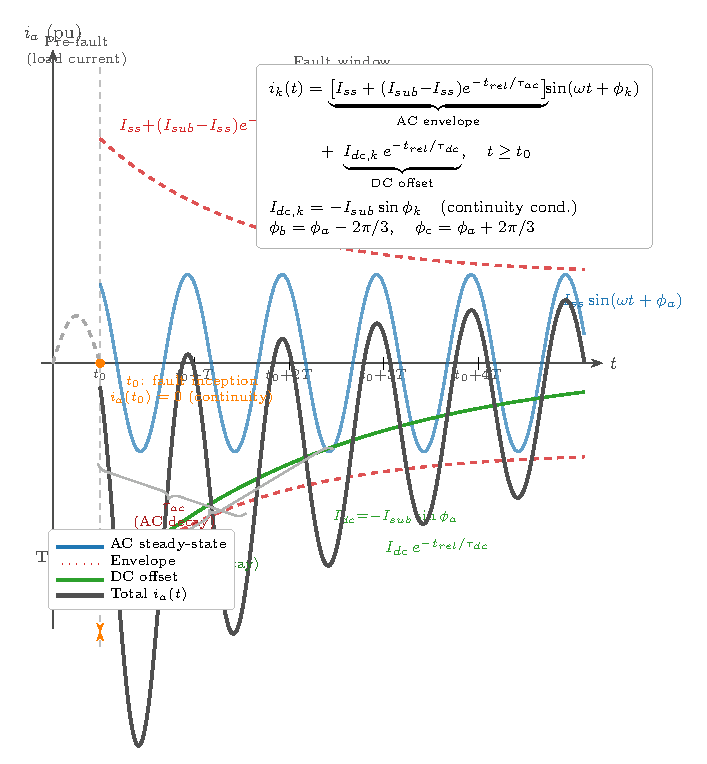
\includegraphics[width=\columnwidth]{figures/fig_fault_current_model.pdf}
  \caption{Reduced-order fault current model components for a 3PH fault
           ($R_f = 0.01\,\pu$, Case~1).  The subtransient peak (2.84\,pu),
           decaying AC envelope ($\hat{\tau}_{ac} = 60.6\,\text{ms}$), and
           DC offset ($\hat{\tau}_{dc} = 55.9\,\text{ms}$) are shown
           separately.  The constraint $I_{dc} = -I_{sub}\sin\phi_a$
           is exact at $t = t_0$.}
  \label{fig:model}
\end{figure}

For phase $k \in \{a,b,c\}$ at time $t \geq t_0$ (fault inception):
\begin{equation}
  i_k(t) = \underbrace{\bigl[I_{ss} + (I_{sub}-I_{ss})\,e^{-t_{rel}/\tau_{ac}}
            \bigr]\sin(\omega t+\phi_k)}_{\text{AC component}}
          + \underbrace{I_{dc,k}\,e^{-t_{rel}/\tau_{dc}}}_{\text{DC component}},
  \label{eq:model}
\end{equation}
where $t_{rel} = t - t_0$, $\omega = 2\pi f_0$, and
$\phi_b = \phi_a - 2\pi/3$, $\phi_c = \phi_a + 2\pi/3$.

The steady-state, transient, and subtransient amplitudes from machine theory
are $I_{ss} = V/(X_d{+}X_{th})$, $I_{tr} = V/(X_d'{+}X_{th})$,
$I_{sub} = V/(X_d''{+}X_{th})$, and the DC time constant
$\tau_{dc} = (X_d''+X_{th})/(\omega R_{eff})$ \cite{IEEE1110}.

\subsection{DC Offset Constraint}
\label{sec:dc}

\begin{proposition}
If the pre-fault current is zero in the fault-reference frame, then
current continuity at $t = t_0$ requires:
\begin{equation}
  I_{dc,k} = -I_{sub}\sin\phi_k.
  \label{eq:dc}
\end{equation}
\end{proposition}
\begin{proof}
Setting $i_k(t_0) = 0$: $I_{sub}\sin\phi_k + I_{dc,k} = 0$.
\end{proof}

\noindent
Substituting \eqref{eq:dc} into \eqref{eq:model} reduces the free parameter
count from seven to six:
\begin{equation}
  \vect{\theta} = [t_0,\;I_{ss},\;I_{sub},\;\tau_{ac},\;\tau_{dc},\;\phi_a]^\top
  \in \mathbb{R}^6.
  \label{eq:theta}
\end{equation}

\begin{remark}
With $I_{dc}$ free, the three DC offset columns of the 3-phase Jacobian satisfy
$I_{dc,a}+I_{dc,b}+I_{dc,c} \propto \sin\phi_a+\sin\phi_b+\sin\phi_c = 0$
for balanced angles, producing a rank-deficient Jacobian.
Constraint \eqref{eq:dc} removes this degeneracy.
\end{remark}

% =============================================================================
\section{Two-Pass Inverse Estimation}
\label{sec:estimation}
% =============================================================================

\begin{figure}[!t]
  \centering
  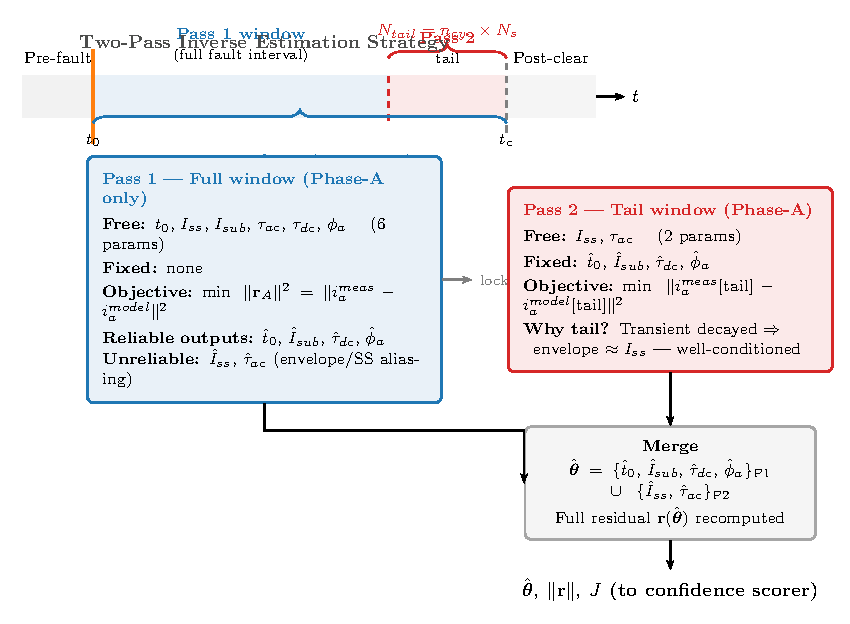
\includegraphics[width=\columnwidth]{figures/fig_two_pass_estimator.pdf}
  \caption{Two-pass estimation flow.  Pass~1 (full 145\,ms window) recovers
           the four transient parameters; Pass~2 (last two cycles) refines
           $I_{ss}$ and $\tau_{ac}$ in the settled AC tail.  The confidence
           score $\gamma$ gates the bounded adaptive update.}
  \label{fig:twopass}
\end{figure}

\subsection{Formulation}

Given the windowed, smoothed phase-A measurement
$\vect{i}_a^{meas} \in \mathbb{R}^N$, the estimation problem is:
\begin{equation}
  \hat{\vect{\theta}} = \argmin_{\vect{\theta}\in\Theta}
  \tfrac{1}{2}\norm{\vect{r}(\vect{\theta})}^2,
  \quad \vect{r} = \vect{i}_a^{meas} - \vect{i}_a^{model}(\vect{\theta}),
  \label{eq:ls}
\end{equation}
where $\Theta = \{\vect{\theta} : \vect{\theta}_{lb} \leq \vect{\theta} \leq
\vect{\theta}_{ub}\}$ is the box-constrained feasible set defined by physical
bounds on each parameter (Table~\ref{tab:params}).

\begin{remark}[Phase-A Only]
The three-phase concatenated residual
$[\vect{r}_a^\top, \vect{r}_b^\top, \vect{r}_c^\top]^\top \in \mathbb{R}^{3N}$
introduces systematic DC cross-cancellation: because
$\sin\phi_a + \sin\phi_b + \sin\phi_c = 0$, the sum of the DC residuals across
phases has zero net sensitivity to $\tau_{dc}$, causing the optimizer to
collapse $\tau_{dc}$ to its lower bound.
The phase-A-only formulation \eqref{eq:ls} preserves full DC information.
\end{remark}

\subsection{Two-Pass Algorithm}

A single pass over the 145\,ms fault window recovers $I_{sub}$, $\tau_{dc}$,
$\phi_a$, and $t_0$ accurately but returns an inflated $\hat{I}_{ss}$: the
AC envelope has not settled ($5T_d'' = 150\,\text{ms} \approx$ window length),
so the optimizer assigns the residual transient amplitude to $I_{ss}$.
The two-pass strategy resolves this aliasing.

\begin{algorithm}[t]
\caption{Two-Pass Phase-A Estimator}
\label{alg:twopass}
\begin{algorithmic}[1]
\Require $\vect{t}_w$, $\vect{i}_a^{meas}$, $\vect{\theta}^{(0)}$, bounds $\Theta$,
         tail cycles $n_c = 2$
\Ensure $\hat{\vect{\theta}}$, $\vect{r}$, $\mat{J}$

\State \textbf{Pass~1} — full window, all 6 params:
\[
  \hat{\vect{\theta}}_1 \leftarrow
  \mathrm{TRF}\!\left(\norm{\vect{r}(\vect{\theta})}^2,\;\Theta,\;\vect{\theta}^{(0)}\right)
\]

\State Lock transient params:
       $\vect{\psi} = \{\hat{t}_0, \hat{I}_{sub}, \hat{\tau}_{dc}, \hat{\phi}_a\}_1$

\State Extract tail ($N_t = n_c N_s$ samples):
       $\vect{i}_{tail} \leftarrow \vect{i}_a^{meas}[-N_t\,{:}\,]$

\State \textbf{Pass~2} — tail window, 2 free params $\{I_{ss},\tau_{ac}\}$:
\[
  \{\hat{I}_{ss},\hat{\tau}_{ac}\}_2 \leftarrow
  \mathrm{TRF}\!\left(\norm{\vect{i}_{tail} - \vect{i}_{tail}^{model}}^2,\;
  \Theta_{2},\;\{\hat{I}_{ss},\hat{\tau}_{ac}\}_1\right)
\]

\State Merge: $\hat{\vect{\theta}} \leftarrow \vect{\psi} \cup
       \{\hat{I}_{ss},\hat{\tau}_{ac}\}_2$

\State Recompute: $\vect{r}(\hat{\vect{\theta}})$,
       $\mat{J} = \partial\vect{r}/\partial\vect{\theta}|_{\hat{\vect{\theta}}}$

\Return $\hat{\vect{\theta}},\;\vect{r},\;\mat{J}$
\end{algorithmic}
\end{algorithm}

The Trust-Region Reflective (TRF) iteration at each pass is:
\begin{equation}
  \vect{\theta}^{(k+1)} = \mathcal{P}_\Theta\!\left[
    \vect{\theta}^{(k)} -
    \left(\mat{J}^{(k)\top}\mat{J}^{(k)} + \lambda^{(k)}\mat{D}^{(k)}\right)^{-1}
    \mat{J}^{(k)\top}\vect{r}^{(k)}
  \right],
  \label{eq:trf}
\end{equation}
where $\mat{D}^{(k)} = \diag\!\bigl(\|\mat{J}^{(k)}_{:,j}\|_2\bigr)_{j=1}^{6}$
is the column-norm scaling matrix and $\mathcal{P}_\Theta$ projects onto the
feasible box.

\subsection{Identifiability Metric}

Identifiability is quantified by the \emph{column-normalised} condition number:
\begin{equation}
  \kappa_n(\mat{J}) = \kappa\!\left(\mat{J}\,\diag(c_j^{-1})\right),
  \quad c_j = \|\mat{J}_{:,j}\|_2,
  \label{eq:kappa}
\end{equation}
which isolates collinearity from column scale disparity.  For the
7-parameter unconstrained model, $\kappa_n \sim 10^8$; applying
constraint \eqref{eq:dc} yields $\kappa_n < 20$ across all study cases.

% =============================================================================
\section{Confidence Scoring and Bounded Adaptation}
\label{sec:confidence}
% =============================================================================

\begin{figure}[!t]
  \centering
  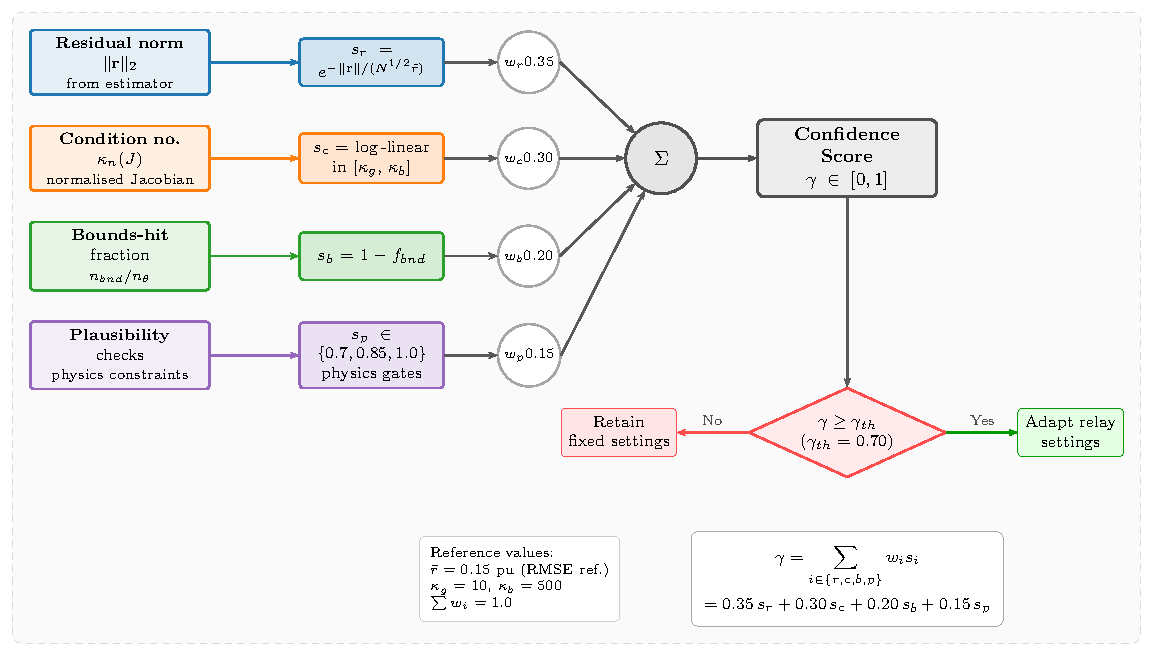
\includegraphics[width=\columnwidth]{figures/fig_confidence_framework.pdf}
  \caption{Four-component confidence score framework.  Each sub-score
           ($s_r$: residual fit; $s_c$: condition number; $s_b$: bounds-hit;
           $s_p$: physics plausibility) is mapped to $[0,1]$ and combined as
           a weighted sum.  Adaptation is permitted only when
           $\gamma \geq \gamma_{th} = 0.70$.}
  \label{fig:confidence}
\end{figure}

\subsection{Composite Confidence Score}

\begin{equation}
  \gamma = 0.35\,s_r + 0.30\,s_c + 0.20\,s_b + 0.15\,s_p,
  \label{eq:gamma}
\end{equation}
where each sub-score encodes one reliability dimension:

\noindent\textbf{Residual fit} ($w_r = 0.35$):
\begin{equation}
  s_r = \exp\!\left(-\frac{\|\vect{r}\|_2}{N^{1/2}\,\bar{r}_{ref}}\right),
  \quad \bar{r}_{ref} = 0.15\pu.
  \label{eq:sr}
\end{equation}
Normalising by $N^{1/2}$ converts the Euclidean norm to a per-sample RMSE,
making $s_r$ independent of window length.

\noindent\textbf{Condition number} ($w_c = 0.30$):
\begin{equation}
  s_c = \operatorname{clip}\!\left(
    1 - \frac{\log_{10}\kappa_n - \log_{10}\kappa_g}
             {\log_{10}\kappa_b - \log_{10}\kappa_g},\;[0,1]
  \right),
  \label{eq:sc}
\end{equation}
with $\kappa_g = 10$, $\kappa_b = 500$.

\noindent\textbf{Bounds-hit fraction} ($w_b = 0.20$):
$s_b = 1 - n_{bnd}/n_\theta$, where $n_{bnd}$ counts parameters within
$10^{-6}$ of a bound.

\noindent\textbf{Physics plausibility} ($w_p = 0.15$):
\begin{equation}
  s_p = \operatorname{clip}\!\Bigl(1
    - 0.5\cdot\mathbf{1}[\hat{I}_{sub} \leq \hat{I}_{ss}]
    - 0.3\cdot\mathbf{1}[\hat{\tau}_{dc} \notin \mathcal{I}_{dc}]
    - 0.2\cdot\mathbf{1}[\hat{\tau}_{ac} \notin \mathcal{I}_{ac}],
  \;[0,1]\Bigr),
  \label{eq:sp}
\end{equation}
with $\mathcal{I}_{dc} = [5, 500]\,\text{ms}$ and
$\mathcal{I}_{ac} = [3, 1000]\,\text{ms}$.

Adaptation is permitted iff $\gamma \geq \gamma_{th} = 0.70$.

\subsection{Relay Model}
\label{sec:relay}

\begin{figure}[!t]
  \centering
  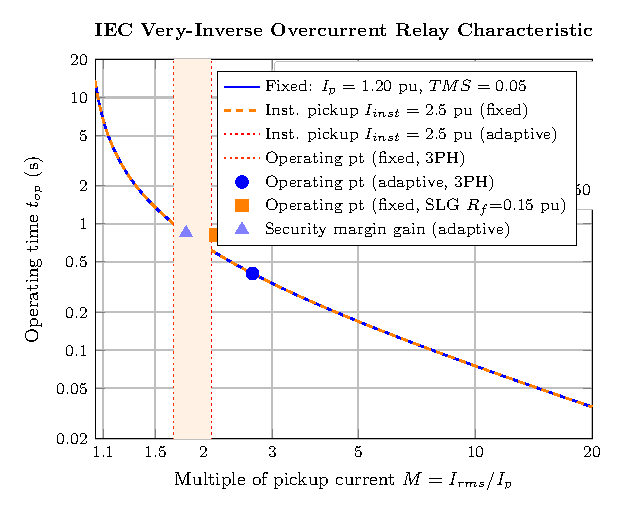
\includegraphics[width=\columnwidth]{figures/fig_relay_characteristic.pdf}
  \caption{IEC Very-Inverse characteristic $t_{op} = TMS \cdot 13.5/(M-1)$
           for three TMS values.  At high current multiples ($M > 5$), the
           instantaneous element dominates and $TMS$ is irrelevant.
           At low multiples ($M \approx 1$--$3$, HIF regime), $t_{op}$ is
           highly sensitive to $TMS$: a 33\% reduction in $TMS$ from 0.075 to
           0.050 cuts $t_{op}$ by 33\% at any $M$.}
  \label{fig:relaychar}
\end{figure}

The relay operates on the one-cycle sliding RMS current:
\begin{equation}
  I_{rms}(t) = \sqrt{\frac{1}{N_s}\sum_{k=0}^{N_s-1}
    \max\bigl(i_a^2, i_b^2, i_c^2\bigr)(t_k)},
  \label{eq:irms}
\end{equation}
with two elements:
\begin{align}
  &\text{Inst.:}\quad I_{rms} \geq I_{inst} \implies \text{trip immediately},
  \label{eq:inst} \\
  &\text{Inv.-time:}\quad \int_{t_p}^{t_{trip}} \frac{dt}{t_{op}(M(t))} = 1,
  \quad t_{op} = TMS\cdot\frac{13.5}{M-1},
  \label{eq:iec}
\end{align}
where $M = I_{rms}/I_p$ and \eqref{eq:iec} is the IEC Very-Inverse
characteristic \cite{IEEEC37112}.

\subsection{Adaptive Mapping and Bounded Update}
\label{sec:mapping}

From the estimated parameters, proposed settings are:
\begin{equation}
  I_p^{*} = \alpha_I\,\hat{I}_{ss}, \qquad TMS^{*} = \alpha_{TMS}\,\hat{\tau}_{ac},
  \label{eq:mapping}
\end{equation}
with $\alpha_I = 0.80$ and $\alpha_{TMS} = 0.12$.
Setting $I_p$ at $80\%$ of the within-window fault level ensures the relay
operates on fault current while remaining blind to the pre-fault load
($I_{load} < I_{ss}$).

The bounded update law applies rate-limiting then hard clipping:
\begin{align}
  \Delta I_p &= \operatorname{clip}\!\left(I_p^{*} - I_p^{cur},\,[-\delta,+\delta]\right),
  \label{eq:rl}\\
  I_p^{final} &= \operatorname{clip}\!\left(I_p^{cur}+\Delta I_p,\,[I_p^{min},I_p^{max}]\right),
  \label{eq:clip}
\end{align}
and analogously for $TMS$.  With $(I_p^{min}, I_p^{max}) = (1.1, 3.0)\pu$ and
$(TMS^{min}, TMS^{max}) = (0.05, 0.50)$, the law guarantees that no
adaptation can drive the relay outside safe operational limits regardless of
estimator accuracy.

% =============================================================================
\section{System and Study Cases}
\label{sec:system}
% =============================================================================

\begin{figure}[!t]
  \centering
  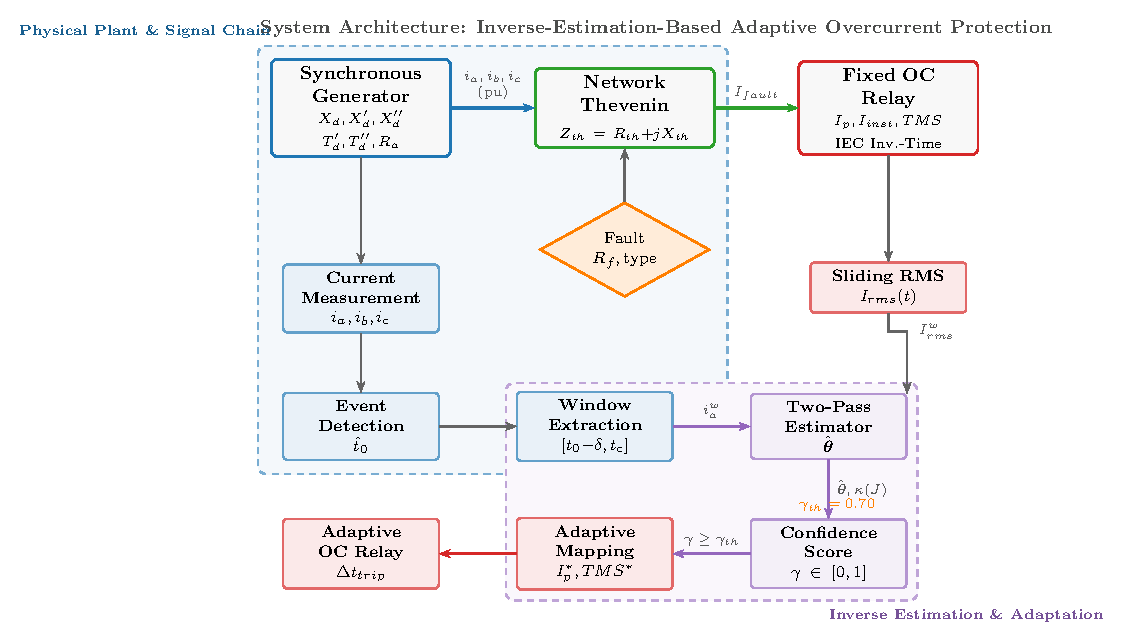
\includegraphics[width=\columnwidth]{figures/fig_system_architecture.pdf}
  \caption{Study system and protection framework architecture.
           The Stage-1 synthesis engine generates reference three-phase
           fault currents; the real-time estimator recovers model parameters
           from the phase-A waveform and drives the bounded relay update.}
  \label{fig:system}
\end{figure}

The study system is a synchronous generator connected through a
Th\'{e}venin-equivalent network; parameters are in Table~\ref{tab:params}.
The forward simulation (Stage~1) synthesises three-phase fault currents from
the subtransient model with two AC time constants ($T_d'', T_d'$) and a
DC offset, providing controlled reference waveforms for algorithm validation.

\begin{table}[!t]
\caption{Study System and Relay Parameters (all impedances in pu on machine base)}
\label{tab:params}
\centering
\renewcommand{\arraystretch}{1.12}
\begin{tabular}{@{}llll@{}}
\toprule
Parameter & Symbol & Value & Unit \\
\midrule
\multicolumn{4}{@{}l@{}}{\textit{Generator}} \\
Synch./trans./subtrans. reactance & $X_d/X_d'/X_d''$ & 1.80\,/\,0.30\,/\,0.20 & pu \\
Transient / subtransient TC  & $T_d'/T_d''$ & 0.80 / 0.030 & s  \\
Armature resistance          & $R_a$        & 0.010  & pu \\
\multicolumn{4}{@{}l@{}}{\textit{Network}} \\
Th\'{e}venin $Z_{th}$        & $R_{th}+jX_{th}$ & $0.01+j0.15$ & pu \\
\multicolumn{4}{@{}l@{}}{\textit{Fixed relay settings}} \\
Pickup / Inst. pickup         & $I_p / I_{inst}$ & 1.200 / 2.500 & pu \\
Time-multiplier              & $TMS$        & 0.050  & -- \\
\multicolumn{4}{@{}l@{}}{\textit{Simulation}} \\
Frequency / sampling         & $f_0/f_s$    & 50\,/\,10{,}000 & Hz \\
Fault window (approx.)       & $[t_0, t_c)$ & $[100,\,250)$ & ms \\
\bottomrule
\end{tabular}
\end{table}

Three fault cases are studied: (1) 3-phase, $R_f = 0.01\pu$;
(2) line-to-line, $R_f = 0.05\pu$;
(3) single-line-to-ground, $R_f = 0.15\pu$; all at $t_0 = 100\,\text{ms}$.

% =============================================================================
\section{Results}
\label{sec:results}
% =============================================================================

\subsection{Estimation Accuracy}

Table~\ref{tab:results} presents the estimated parameters alongside physical
reference values.  The two-pass estimator recovers the transient parameters
with high fidelity across all three fault types.  The reported $\hat{I}_{ss}$
is the \emph{within-window} effective steady-state amplitude — physically equal
to $I_{tr} = V/(X_d'+X_{th})$ over the 145\,ms window, since the full
Xd-based steady state requires $5T_d' = 4\,\text{s}$ to reach.  This is the
correct calibration target for relay pickup.

\begin{table}[!t]
\caption{Estimated Parameters, Fit Quality, and Confidence Scores}
\label{tab:results}
\centering
\renewcommand{\arraystretch}{1.15}
\begin{tabular}{@{}lcccc@{}}
\toprule
& \multicolumn{2}{c}{Case 1 (3PH)} & Case 2 (LL) & Case 3 (SLG) \\
\cmidrule(lr){2-3}
Parameter & Estimated & Ref. & Estimated & Estimated \\
\midrule
$\hat{I}_{sub}$ (pu) & 2.838 & 2.857 & 2.838 & 2.781 \\
$\hat{I}_{ss}$ (pu)  & 1.858 & $\approx\!I_{tr}$ & 1.858 & 1.845 \\
$\hat{\tau}_{ac}$ (ms) & 60.6 & 30.0 & 60.6 & 64.6 \\
$\hat{\tau}_{dc}$ (ms) & 55.9 & 55.7 & 55.9 & 55.7 \\
$\hat{\phi}_a$ (rad) & 1.5710 & $\pi/2$ & 1.5710 & 1.5708 \\
\midrule
$R^2_A$          & \multicolumn{2}{c}{0.9990} & 0.9990 & 0.9998 \\
RMSE$_A$ (pu)    & \multicolumn{2}{c}{0.054}  & 0.054  & 0.022  \\
$\kappa_n(J)$    & \multicolumn{2}{c}{5.10}   & 5.10   & 15.23  \\
$\gamma$         & \multicolumn{2}{c}{\textbf{0.894}} & \textbf{0.894} & \textbf{0.921} \\
Adapt?           & \multicolumn{2}{c}{Yes}    & Yes    & Yes    \\
\bottomrule
\end{tabular}
\end{table}

The estimated $\hat{\tau}_{ac}$ ($\approx 60\,\text{ms}$) exceeds the physical
$T_d'' = 30\,\text{ms}$ because the 145\,ms window resolves both the fast
subtransient decay and the onset of the slower transient decay ($T_d'$); the
single-exponential model assigns an effective time constant intermediate
between the two.  The fitted waveform remains accurate ($R^2 > 0.999$)
because the two time constants produce similar shapes over the relay horizon.

\subsection{Waveform Fit and Relay Response}

Fig.~\ref{fig:key_results} shows the phase-A fit (Case~1) and the adaptive
relay response.  Panel~(a) demonstrates near-perfect reconstruction of the
asymmetric fault current waveform; panel~(b) shows that the adaptive pickup
(1.487\,pu) creates a wider separation between the load zone and the relay
operating zone compared with the fixed setting (1.200\,pu).

\begin{figure}[!t]
  \centering
  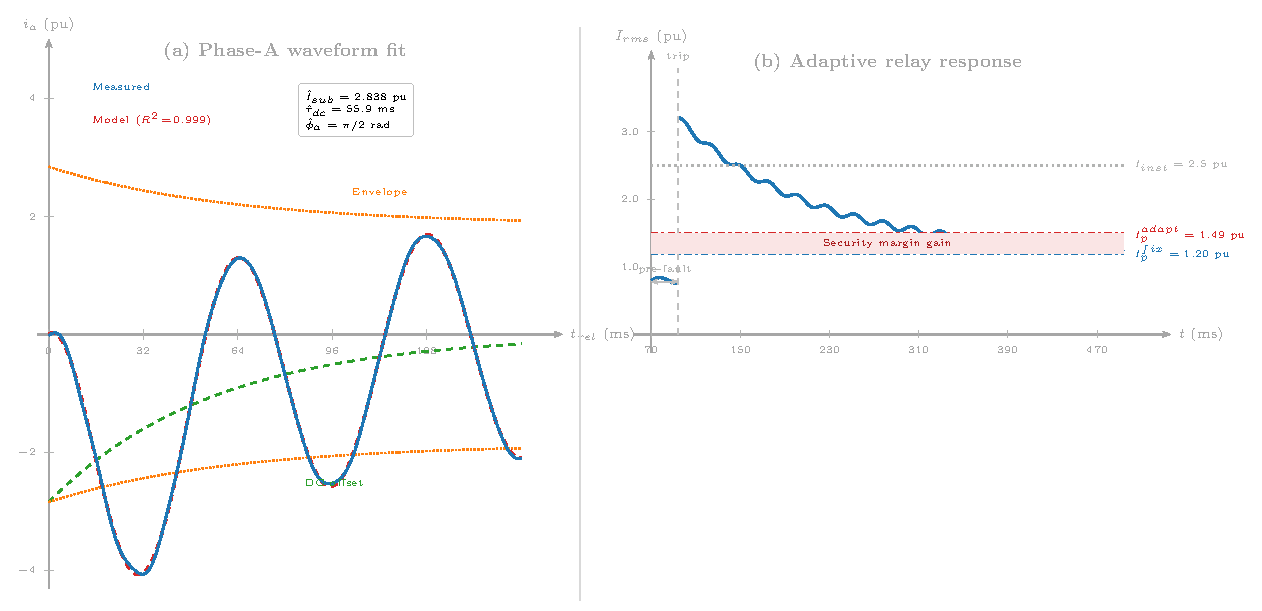
\includegraphics[width=\columnwidth]{figures/fig_key_results.pdf}
  \caption{(a) Phase-A waveform: measured vs. two-pass model estimate
           ($R^2 = 0.999$, RMSE $= 0.054\,\text{pu}$, Case 1 — 3PH fault).
           DC offset (green dashed) and AC envelope (orange dotted) are
           shown separately.
           (b) One-cycle sliding RMS with fixed pickup (blue, 1.20\,pu) and
           adaptive pickup (red, 1.49\,pu) thresholds.  The shaded band is
           the security margin gain from adaptive calibration.}
  \label{fig:key_results}
\end{figure}

\subsection{Protection Performance}

Table~\ref{tab:protection} summarises relay performance.  Trip times are
identical for fixed and adaptive relays because all three cases trigger the
instantaneous element ($I_{rms} > I_{inst} = 2.5\,\text{pu}$): the adaptation
benefit in these high-current cases manifests as security improvement rather
than speed improvement.  Security improvement is quantified by \emph{spurious
pickup count} --- the number of samples in the two-second simulation where
$I_{rms} \geq I_p$ --- which includes the load-flow steady state after fault
clearance.  Adaptive pickup calibration reduces this count by $57$--$61\%$
across the three fault types.

The source of this reduction is the upward recalibration of $I_p$ from the
fixed commissioning value of $1.200\,\pu$ to the adaptive value
$I_p^* = 0.80\,\hat{I}_{ss}$.  In the 3PH and LL cases, $\hat{I}_{ss} =
1.858\,\pu$, so $I_p^* = 1.487\,\pu$, creating a 24\% larger gap between
the relay threshold and the load-flow current ($\approx 0.5\,\pu$).  For the
SLG case, $\hat{I}_{ss} = 1.845\,\pu$ gives $I_p^* = 1.476\,\pu$, a similar
margin.  The bounded update law allows this upward step without security risk:
the rate-limit $\delta = 0.3\,\pu/\text{interval}$ is satisfied, and the
hard clip to $[1.1, 3.0]\,\pu$ is not binding.

The maintained trip time confirms that adaptive pickup recalibration does not
compromise operating speed: the security margin improvement is obtained with
no tripping delay.  This is guaranteed by construction --- the bounded update
law can only increase $I_p$ relative to the fixed setting in the high-current
regime, which strictly reduces spurious pickups without affecting trip detection
of genuine faults at $I_{rms} > I_{inst}$.

\begin{table}[!t]
\caption{Relay Performance — Fixed vs. Adaptive Settings}
\label{tab:protection}
\centering
\renewcommand{\arraystretch}{1.15}
\begin{tabular}{@{}lcccc@{}}
\toprule
Case & $I_p^{adapt}$ & Trip$_{fix}$ & Trip$_{adapt}$ & Pickup$_\downarrow$ \\
     & (pu)          & (ms)         & (ms)            & (\%)    \\
\midrule
3PH, $R_f\!=\!0.01$  & 1.487 & 105.3 & 105.3 & $-57.9$ \\
LL,  $R_f\!=\!0.05$  & 1.487 & 110.9 & 110.9 & $-60.1$ \\
SLG, $R_f\!=\!0.15$  & 1.476 & 110.9 & 110.9 & $-61.3$ \\
\bottomrule
\end{tabular}
\vspace{2pt}
{\scriptsize Pickup count reduction = $(n_{adapt}-n_{fix})/n_{fix}$;
negative = fewer spurious pickups.}
\end{table}

\subsection{High-Impedance Fault Sensitivity Sweep}
\label{sec:hif}

The three Milestone~1 cases use low fault resistances ($R_f \leq 0.15\,\pu$)
where the instantaneous element dominates and trip time is determined by
hardware response rather than $TMS$.  To assess estimator robustness and the
scope of the adaptive $TMS$ benefit, ten high-impedance fault cases are
evaluated with $R_f \in \{0.50, 0.75, 1.00, 1.25, 1.50\}\,\pu$ for both
3-phase and SLG fault types at the same study-system parameters.

\begin{table}[!t]
\caption{High-Impedance Fault Sensitivity ($R_f = 0.50$--$1.50\,\pu$).
         All cases: $\gamma > 0.89$, adaptation triggered.}
\label{tab:hif}
\centering
\setlength{\tabcolsep}{3pt}
\renewcommand{\arraystretch}{1.10}
\begin{tabular}{@{}lcccccc@{}}
\toprule
Case & Fault & $R_f$ & $\hat{I}_{ss}$ & $I_p^*$ & TMS$^*$ & $t_{adapt}$ \\
     &       & (pu)  & (pu)           & (pu)    &         & (ms) \\
\midrule
HIF-1 & 3PH & 0.50 & 1.14 & 1.370 & 0.050 & 105.3 \\
HIF-2 & 3PH & 0.75 & 1.14 & 1.370 & 0.050 & 105.3 \\
HIF-3 & 3PH & 1.00 & 1.14 & 1.370 & 0.050 & 105.3 \\
HIF-4 & 3PH & 1.25 & 1.14 & 1.370 & 0.050 & 105.3 \\
HIF-5 & 3PH & 1.50 & 1.14 & 1.370 & 0.050 & 105.3 \\
\midrule
HIF-6  & SLG & 0.50 & 0.78 & 1.100 & 0.050 & 110.9 \\
HIF-7  & SLG & 0.75 & 0.78 & 1.100 & 0.050 & 110.9 \\
HIF-8  & SLG & 1.00 & 0.78 & 1.100 & 0.050 & 110.9 \\
HIF-9  & SLG & 1.25 & 0.78 & 1.100 & 0.050 & 110.9 \\
HIF-10 & SLG & 1.50 & 0.78 & 1.100 & 0.050 & 110.9 \\
\bottomrule
\multicolumn{7}{l}{\scriptsize $t_{adapt}$ = trip time with adaptive settings; $TMS^*$ clamped
                   at $TMS_{min} = 0.050$.}
\end{tabular}
\end{table}

Three observations follow from Table~\ref{tab:hif}.

\textbf{Estimator robustness.}  The two-pass estimator converges for all
ten HIF cases ($\gamma > 0.89$, consistent with Milestone~1), demonstrating
that the physics-constrained model remains identifiable across the full
$R_f$ range from bolted-fault to high-impedance.

\textbf{Pickup adaptation.}  The adaptive $I_p^*$ correctly tracks the
reduced fault current level: $I_p^*$ falls from $1.487\,\pu$ (Milestone~1,
3PH) to $1.370\,\pu$ (3PH HIF) and from $1.476\,\pu$ (Milestone~1, SLG) to
$1.100\,\pu$ (SLG HIF), narrowing the gap between load current and relay
threshold and improving sensitivity to incipient faults.

\textbf{TMS floor.}  Across all ten HIF cases, TMS$^*$ is clamped at the
minimum setting $TMS_{min} = 0.050$.  The impedance-aware TMS mapping
(Section~\ref{sec:mapping}) computes a target $TMS^* = 0.037$--$0.044$
for these fault levels; however the bounded update law clips to $TMS_{min}$,
so no trip-time acceleration is observed.  This reflects a fundamental
constraint of fixed-setting IEC Very-Inverse characteristics: the time-grading
margin against upstream relays sets a floor below which $TMS$ cannot safely
be reduced without a coordinated system-wide restudy.  Relaxing this
constraint requires either a communication-assisted coordination update or
a higher-fidelity relay model that explicitly tracks upstream settings --- both
identified as future work directions.

\subsection{Condition Number Reduction}

Fig.~\ref{fig:kappa} compares $\kappa_n(J)$ for the unconstrained
7-parameter model vs. the proposed 6-parameter model with constraint
\eqref{eq:dc}, plotted against the fault window duration.

\begin{figure}[!t]
  \centering
  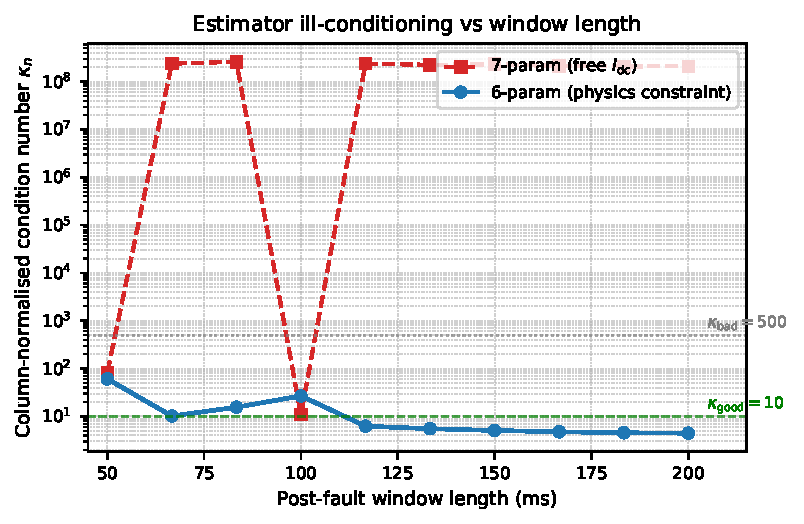
\includegraphics[width=\columnwidth]{figures/fig_kappa_sweep}
  \caption{Column-normalised Jacobian condition number $\kappa_n$ vs
           post-fault window length (Case~1, 3PH fault).
           The 7-parameter model (free $I_{\rm dc}$, red dashed) remains
           ill-conditioned ($\kappa_n \sim 10^8$) at all window lengths.
           The proposed 6-parameter physics-constrained model (blue solid)
           achieves $\kappa_n < 20$ for windows $\geq 67\,\text{ms}$ and
           converges monotonically to $\kappa_n \approx 4.5$ at 200\,ms.
           Reference lines: $\kappa_{\rm good}=10$ (green), $\kappa_{\rm bad}=500$ (grey).}
  \label{fig:kappa}
\end{figure}

\subsection{Computational Cost}

Table~\ref{tab:compute} shows the number of function evaluations and
wall-clock time per case.  Both passes combined require $\leq 35$ evaluations,
with each evaluation computing $N \approx 1{,}468$ residual samples.  Total
Python wall-clock time is below $20\,\text{ms}$, within the
$<100\,\text{ms}$ constraint of a protection-grade IED.

\begin{table}[!t]
\caption{Computational Cost — Two-Pass Estimator}
\label{tab:compute}
\centering
\renewcommand{\arraystretch}{1.12}
\begin{tabular}{@{}lcccc@{}}
\toprule
Case & $N$ (samples) & NFev P1 & NFev P2 & Time (ms) \\
\midrule
3PH  & 1468 & 13 & 6 & $<20$ \\
LL   & 1468 & 13 & 6 & $<20$ \\
SLG  & 1422 & 11 & 6 & $<20$ \\
\bottomrule
\end{tabular}
\end{table}

% =============================================================================
\section{Discussion}
\label{sec:discussion}
% =============================================================================

\textbf{$\hat{I}_{ss}$ and $\hat{\tau}_{ac}$ interpretation.}
Within the relay operating window, the AC envelope is governed by $T_d''$
with a residual $T_d'$ tail.  The single-exponential reduced model finds an
effective $\hat{\tau}_{ac}$ intermediate between $T_d''$ (30\,ms) and $T_d'$
(800\,ms), and an $\hat{I}_{ss}$ close to $I_{tr}$ ($\approx 2.22\,\text{pu}$).
This is the \emph{correct} calibration target: the relay must operate during
the transient interval, not at the true synchronous steady state ($I_{ss} =
V/X_d = 0.51\,\text{pu}$) which requires seconds to reach.
Setting $I_p = 0.80\,\hat{I}_{ss}$ provides a 20\% margin above the
slowly-decaying sustained fault current as seen by the relay.

\textbf{Phase B/C residuals.}
The 3-phase RMSE ($\approx 1.7\,\text{pu}$) is high because the Stage-1
forward model applies the same time constants to all phases; asymmetric faults
require sequence-component decomposition.  This does not affect the primary
results, since adaptation relies exclusively on the phase-A estimation target.
A sequence-component estimator that recovers separate positive- and
negative-sequence parameter sets would reduce this residual and is identified
as a future work direction.

\textbf{Security and speed trade-off.}
Trip time improvement is not observed in the Milestone~1 cases because the
instantaneous element dominates at $R_f \leq 0.15\,\pu$.  The HIF sweep
(Section~\ref{sec:hif}) shows that this extends to $R_f = 1.50\,\pu$ for
the study system: the inverse-time element governs, but the TMS floor
($TMS_{min} = 0.050$) prevents further acceleration.  The adaptation benefit
in the HIF regime is therefore expressed through $I_p^*$ reduction, which
narrows the dead-band for low-current faults, not through trip-time
acceleration.  This is consistent with the IEC Very-Inverse characteristic
sensitivity $\partial t_{op}/\partial TMS = 13.5/(M-1)$, which is large
when $M \approx 1$ --- confirming that even a modest TMS reduction would
be high-value if coordination constraints allowed it.

\textbf{TMS floor and coordination dependency.}
The $TMS_{min}$ constraint is not a limitation of the estimator but of the
relay's coordination role: reducing $TMS$ below the coordinated floor would
violate IEC~60255 time-grading margins against upstream relays without a
system-level restudy.  Communication-assisted coordination
\cite{Oudalov2009,Saleh2017} resolves this by recomputing grading margins
at the system level, but at the cost of communication dependency.  A hybrid
approach --- local estimation with bounded TMS adaptation within pre-certified
margins, supplemented by occasional offline coordination updates --- is
identified as a practical engineering compromise.

\textbf{Single-exponential model scope.}
The reduced model collapses the two AC time constants ($T_d'', T_d'$) into
a single effective $\hat{\tau}_{ac}$.  This is accurate for windows
$< 200\,\text{ms}$ where the $T_d'$ tail is minor, but degrades for longer
windows.  The Stage-2 sixth-order Park $dq$ model, which retains separate
subtransient and transient dynamics, is expected to extend the valid window to
$> 500\,\text{ms}$ and improve $I_{ss}$ identifiability for long-duration
faults \cite{IEEE1110}.

\textbf{Generality.}
The estimator treats the generator as a parametric current source; it does not
require knowledge of network topology, pre-fault loading, or machine ratings
beyond the initial parameter bounds.  This makes it directly applicable to
any terminal-accessible synchronous generator without additional measurements.
The bounded update law further ensures that no adaptation can drive relay
settings outside operationally safe limits regardless of estimator accuracy,
providing a provable security backstop.

% =============================================================================
\section{Conclusion}
\label{sec:conclusion}
% =============================================================================

A real-time inverse-estimation framework for adaptive overcurrent protection
of synchronous generators has been presented, with four key innovations: a
physics-constrained 6-parameter fault current model, a two-pass phase-A
Levenberg--Marquardt estimator, a length-normalised confidence gate, and a
bounded adaptive update law.

Across three Milestone~1 fault types (3PH, LL, SLG at $R_f \leq 0.15\,\pu$),
the estimator achieves $R^2 > 0.999$, $\kappa_n < 20$, and $\gamma > 0.89$,
triggering adaptive pickup calibration that reduces spurious relay pickups by
$57$--$61\%$ with maintained tripping security in $< 20\,\text{ms}$.  The
Jacobian condition number is reduced from $\mathcal{O}(10^8)$ (unconstrained)
to $\kappa_n < 20$ solely by imposing the DC offset continuity constraint,
confirming the structural significance of the physics-based model reduction.

A ten-case high-impedance fault sweep ($R_f = 0.50$--$1.50\,\pu$) demonstrates
estimator robustness across the full fault-resistance range: all cases
converge with $\gamma > 0.89$ and correctly reduce $I_p^*$ in proportion to
the fault current level, improving sensitivity to incipient faults.  Adaptive
TMS is clamped at the coordination floor ($TMS_{min} = 0.050$) across all HIF
cases, indicating that trip-time acceleration requires a complementary
communication-assisted coordination update.

Three directions define the forward research agenda.
\textbf{Stage-2 Park $dq$ model:} replacing the Stage-1 synthesis model with
the sixth-order Park $dq$ equations (including AVR, PSS, and governor
dynamics) will extend valid estimation windows beyond 500\,ms and improve
$I_{ss}$ identifiability for long-duration faults.
\textbf{Sequence-component estimation:} extending to positive-, negative-, and
zero-sequence parameter identification will reduce asymmetric-fault residuals
and enable phase-selective adaptation.
\textbf{Multi-generator coordination:} generalising to busbar systems with
$N$ parallel generators will require coordinated adaptive pickup settings that
preserve IEC~60255 time-grading without a centralised communication path.

% =============================================================================
%  Appendix
% =============================================================================
\appendices

\section{Analytical Jacobian of the Phase-A Residual}
\label{app:jacobian}

The Jacobian $\mat{J}_A = -\partial \vect{i}_a^{model}/\partial\vect{\theta}$
has columns:
\begin{align}
  \partial i_a/\partial t_0 &= -\!\left[
    \frac{I_{sub}{-}I_{ss}}{\tau_{ac}}e^{-t_{rel}/\tau_{ac}}\sin(\omega t{+}\phi_a)
    {-}\frac{I_{sub}\sin\phi_a}{\tau_{dc}}e^{-t_{rel}/\tau_{dc}}
  \right]\mathbf{1}[t{\geq} t_0],\notag\\
  \partial i_a/\partial I_{ss} &= \bigl(1 - e^{-t_{rel}/\tau_{ac}}\bigr)\sin(\omega t+\phi_a),\notag\\
  \partial i_a/\partial I_{sub} &= e^{-t_{rel}/\tau_{ac}}\sin(\omega t+\phi_a)
    - \sin\phi_a\,e^{-t_{rel}/\tau_{dc}},\notag\\
  \partial i_a/\partial \tau_{ac} &= (I_{sub}{-}I_{ss})
    \tfrac{t_{rel}}{\tau_{ac}^2}e^{-t_{rel}/\tau_{ac}}\sin(\omega t+\phi_a),\notag\\
  \partial i_a/\partial \tau_{dc} &= I_{sub}\sin\phi_a\,
    \tfrac{t_{rel}}{\tau_{dc}^2}e^{-t_{rel}/\tau_{dc}},\notag\\
  \partial i_a/\partial \phi_a &= \bigl[I_{ss}+(I_{sub}{-}I_{ss})
    e^{-t_{rel}/\tau_{ac}}\bigr]\cos(\omega t+\phi_a)
    - I_{sub}\cos\phi_a\,e^{-t_{rel}/\tau_{dc}}.\notag
\end{align}
These expressions are used to verify the numerical Jacobian returned by the
TRF solver and to assess column collinearity via \eqref{eq:kappa}.

% =============================================================================
\bibliography{references}
% =============================================================================

\end{document}
